\chapter{Optimizing the synthesis of monodisperse colloidal spheres}
\label{ch:synthesis}

\section{Introduction}

The earliest reference to synthetic emulsion polymerization dates back to
1909 \cite{bayer1909,finch03} to a patent awarded to Felix Hoffmann and
co-workers at Farbenfabriken Bayer for their pioneering work in producing
synthetic latex.
Techniques for polymerizing emulsions have progressed through
intuitive leaps guided by fundamental principles of chemistry
and physics.  Quite often, the importance of particular chemical
or physical conditions to the outcome are gauged once
synthesis is complete, and requires multiple orthogonal measurement
techniques. Examples include measurements of the particles' size distribution,
their surface texture, and their porosity.

Holographic particle
characterization can streamline this analysis by providing particle-resolved assays
of samples' size distributions and composition rapidly and with
minimal sample preparation.

Holographic assays provide information that is useful for designing synthetic
pathways and can help to detect and diagnose deficiencies. These measurements
can proceed rapidly enough, moreover, to provide real-time feedback during
synthesis. We illustrate these capacities by analyzing the synthesis of a
particularly interest colloidal suspension.

In this chapter we use holographic particle characterization
to explore the role of stoichiometry, initiator choice, and
agitation conditions on the synthesis of monodisperse spheres of
\num{3}-methacryloxypropyltrimethoxysilane (TPM) \cite{vanderwel17},
a model system with increasingly widespread applications
in soft-matter research \cite{sacanna11,liu16,vanderwel18}.
We employ holographic particle characterization
in tandem with conventional particle characterization
techniques to identify factors that 
influence size selection, polydispersity, and surface texture.
Complementary analysis serves to validate results obtained by
HPC.

\section{Synthesizing TPM spheres}
% FIXME: Possibly meld the previous paragraph and the next.%

TPM spheres are a particularly useful model system for colloidal studies.
A comparatively straightforward synthesis readily produces monodisperse spheres
with selective sizing between from a few hundred nanometers to a few micrometers
\cite{liu16}.
Unlike the better-known syntheses polystyrene \cite{goodwin1974} and silica \cite{stober68},
TPM particles require no specialized equipment or inert environment necessary.
However, there are many parameters in the synthesis that can affect the average size and refractive
index for a synthesized population. This chapter describes how holographic particle
characterization can guide the synthesis of TPM spheres by elucidating how
synthesis conditions affect the properties of synthesized particles.
Our work builds on the work of van der Wel \emph{et. al} \cite{vanderwel17} that
uses conventional characterization techniques to systematically
characterize the emulsion polymerization protocol for TPM spheres.

Our procedure for synthesizing TPM spheres is described in section
\ref{ssec:synthesizing_tpm} with the
exception of initiator choice. We reiterate the synthesis protocol
here to underscore the conditions we varied and to enumerate the
\num{32} samples of droplets and polymerized spheres we analyzed.
A detailed account of the polymer chemistry underlying this
protocol is provided in Ref.~\cite{vanderwel17}.

\subsection{Emulsion polymerization}
\label{ssec:polymerization}
Controlling the size, monodispersity, and composition of colloidal spheres is crucial
for many applications including colloidal crystallization \cite{pusey87} and micrometer scale
self-assembly \cite{sacanna11}. In this study 
we investigate the influence of stir rate, concentration of ammonium chloride,
concentration of TPM oil, and radical initiator choice on the size and refractive index
of the manufactured particles. To do so, we prepared numerous batches of TPM particles
with independent deviations from the above synthesis protocol and
characterized the resulting particles with holographic particle characterization.

The synthesis begins with the formation of an emulsion of monodisperse TPM droplets.
Monomeric TPM, ((3-(Trimethoxysilyl)propyl methacrylate, \SI{98}{\percent}, Sigma Aldrich)
which is insoluble in water, is added to a basic environment
(pH $>$ \num{9}) of ammonium chloride (\SI{29}{\percent}) in water.
The monomers undergo hydrolysis in water and become water soluble. 
In a basic environment, these hydrolyzed monomers form insoluble 
oligomers. As the suspension is stirred, the oligomers condense 
homogeneously into monodisperse droplets that continue to grow as more oligomers form.
After \num{2} hours, the abundance of free hydrolyzed monomer is depleted
causing oligomerization to halt and therefore droplet growth to cease.
The emulsion is then heated to \SI{80}{\degreeCelsius} and a free radical 
initiator is introduced to polymerize the droplets and form solid spheres.

The dissociation of ammonium chloride in water leads to the production of ammonia
gas,which escapes the solution lessening its pH.
To mitigate this effect, emulsion formation is completed in a closed vial.
Additionally we use identical \SI{12}{\milli\liter} vials to produce \SI{5}{\milli\liter}
of colloidal suspension in each synthesis so that the amount of enclosed air, and therefore
loss in pH, is consistent across samples. Identical stir bars are used for all syntheses
to ensure consistent flow properties.

\subsection{Holographic particle characterization}

We perform holographic characterization measurements with a Spheryx xSight,
a commercial holographic particle characterization system
that automates the methods described in the previous chapters.
The xSight flows a colloidal suspension through the observation volume of a conventional microscope
and illuminates the suspension with a laser operating at a vacuum wavelength of \SI{532}{\nm}.
The proprietary software and hardware implemented in
the instrument yield the size and refractive index for each observed colloidal spheres and
does so in a fraction of the time we typically spend analyzing an experimental video.
Because we are only interested in collecting population statistics for the size and refractive
index of our colloidal systems, we utilize the xSight rather than our custom-built microscope.

The xSight analyzes colloidal dispersions with particle number densities below 
\SI{E6}{\milli\liter^{-1}} to reduce the occurrence of overlapping holograms.
This is consistent with our discussion in section \ref{ssec:sample_prep}.
The emulsification polymerization process described in section \ref{ssec:polymerization}
produces a sample with a number density of \SI{E10}{\milli\liter^{-1}}.
We therefore dilute each of our samples by a factor of \SI{E4}{} with
deionized water.
%We utilized xCells, the flows cells designed for the xSight, with each flow
%analyzing \SI{3}{\micro\liter} of sample passing through a \SI{50}{\um} deep observation volume;
%this provides us with scattering information of a few thousand colloidal spheres per sample.

We analyze \SI{3}{\micro\liter} of each sample by pipetting the diluted dispersion into an
xCell sample cell and loading the xCell into the xSight. The xSight draws the fluid through
the xCell's \SI{50}{\um} deep observation volume. A ten-minute measurement provides us with
characterization data for a few thousand colloidal spheres per sample.

\begin{figure}
    \centering
    \includegraphics[width=\columnwidth]{example_poiseuille_fit}
    \caption{The measured flow profile of particles streaming through the xCell.
      (a)  A diagram of the observed Poiseuille flow.\protect\footnotemark 
      (b) Scatter plot of average particle height and average velocities; each
      dot represents a single micrometer scatterer. Color denotes the density of
      observations. The fit to a parabolic flow profile is illustrated with a dashed
      blue line. (c) Scatter plot of data after filtering observations deviating
      from the parabolic profile.}
    \label{fig:flow_prof}
\end{figure}

\footnotetext{The focal plane is only \SI{90}{\um} below the lower sample-xCell interface:
  a to-scale diagram would depict the focal plane inside the lower xCell wall.}
The dilute suspension is pumped between the stationary walls of the xCell.
The resulting fluid flow takes on a parabolic profile known as a Poiseuille flow.
As the system is in a low-Reynolds number flow, every colloidal sphere traces
the flow of the fluid.
As illustrated in Fig.~\ref{fig:flow_prof}(a), the xCell's walls are located
at \SI{90}{\um} and \SI{150}{\um} relative to the xSight's focal plane.
Because the xSight records the mean $z$-position and mean 
velocity of all multiply-imaged scatterers, we are able to fit the flow
profile to a Poiseuille flow as depicted in Fig.~\ref{fig:flow_prof}(b).
The majority of observations fall neatly onto the parabolic profile. 
Some fits however deviate markedly. Presumably these data result from fitting
false positive detections of overlapping holograms.
We suppress these erroneous features by filtering data that deviate from
the parabolic profile by more than one median absolute deviation
as depicted in Fig.~\ref{fig:flow_prof}(c).

\subsection{Orthogonal validation methods}

We used scanning electron microscopy to provide baseline estimates of the
particles to compare against holographic characterization measurements.
Each sample of polymerized spheres were imaged with a MERLIN (Carl Zeiss) field
emission scanning electron microscope (SEM).
Typical images are provided in Fig.~\ref{fig:sem_stir_rate}(a).
SEM images provide a visual check on the sample's uniformity
and can be used to estimate the colloidal spheres' diameter. While a well calibrated scanning
electron microscope provides \num{1} to \SI{10}{\nm} resolution of features, sample
preparation, particularly vacuum decompression and sputter coating, can shrink or
even swell the sample \cite{yamada85,jung02}. The liquid TPM droplets
are not amendable to SEM analysis.

A common method for determining the refractive index of colloidal particles
requires index matching the particles to a solution with a known refractive index.
This procedure requires dispersing the particles in a solution and therefore
assumes that the solution does not chemically interact with the particles
and does not cause appreciable swelling.  Ref.~\cite{vanderwel17} estimated the
refractive index to be between $\num{1.512}$ and $\num{1.513}$ by index matching
to a solution of pyridine ($n = \SI{1.509}{}$) and \num{2}- ethylhexyl \num{4}-methoxycinnamate
($n = \SI{1.545}{}$). We instead estimated the refractive index of polymerized TPM spheres
from measurements of the refractive index of several dense suspensions of TPM spheres
dispersed in water. For most colloidal suspensions \cite{alexander81}, the refractive index
depends linearly on the volume fraction of particles. With measurements of the refractive
index at multiple volume fractions, we can accurately estimate the refractive index of
TPM particles. 

\section{Results}
\subsection{Effect of stir rate}

Stirring the sample while the oligomers condense into droplets suppresses coalescence and
promotes homogeneous nucleation by uniformly dispersing the hydrolyzed monomer and droplet
nuclei. %%FIXME CHECK THIS STATEMENT.
The effect of stir rate on the resulting particle size is, however, less clear;
we investigated the influence of stir rate by producing \num{4} sets of TPM emulsions.
In four identical vials with identical stir bars, we placed \SI{15}{\milli\liter} of 
\SI{29}{\percent} ammonia followed by \SI{200}{\micro\liter} of TPM 
monomer to \SI{5}{\milli\liter} of DI water. The four samples were then stirred 
using magnetic stir plates set at \num{500}, \num{700}, \num{900}, and
\SI{1100}{\minute^{-1}} for \SI{2}{\hour}. 
The droplets were then polymerized by adding
\num{2},\num{2}'-azobis(\num{2}-methylpropionitrile, Sigma Aldrich) (AIBN) as a radical initiator and %FIXME: Lot number of AIBN?
heating the sample to \SI{80}{\celsius} for \SI{2}{\hour}.
We prepared a sample of unpolymerized droplets and a sample of polymerized TPM spheres
at each of the four spin rates, for a total of eight samples.

\begin{figure}
    \centering
    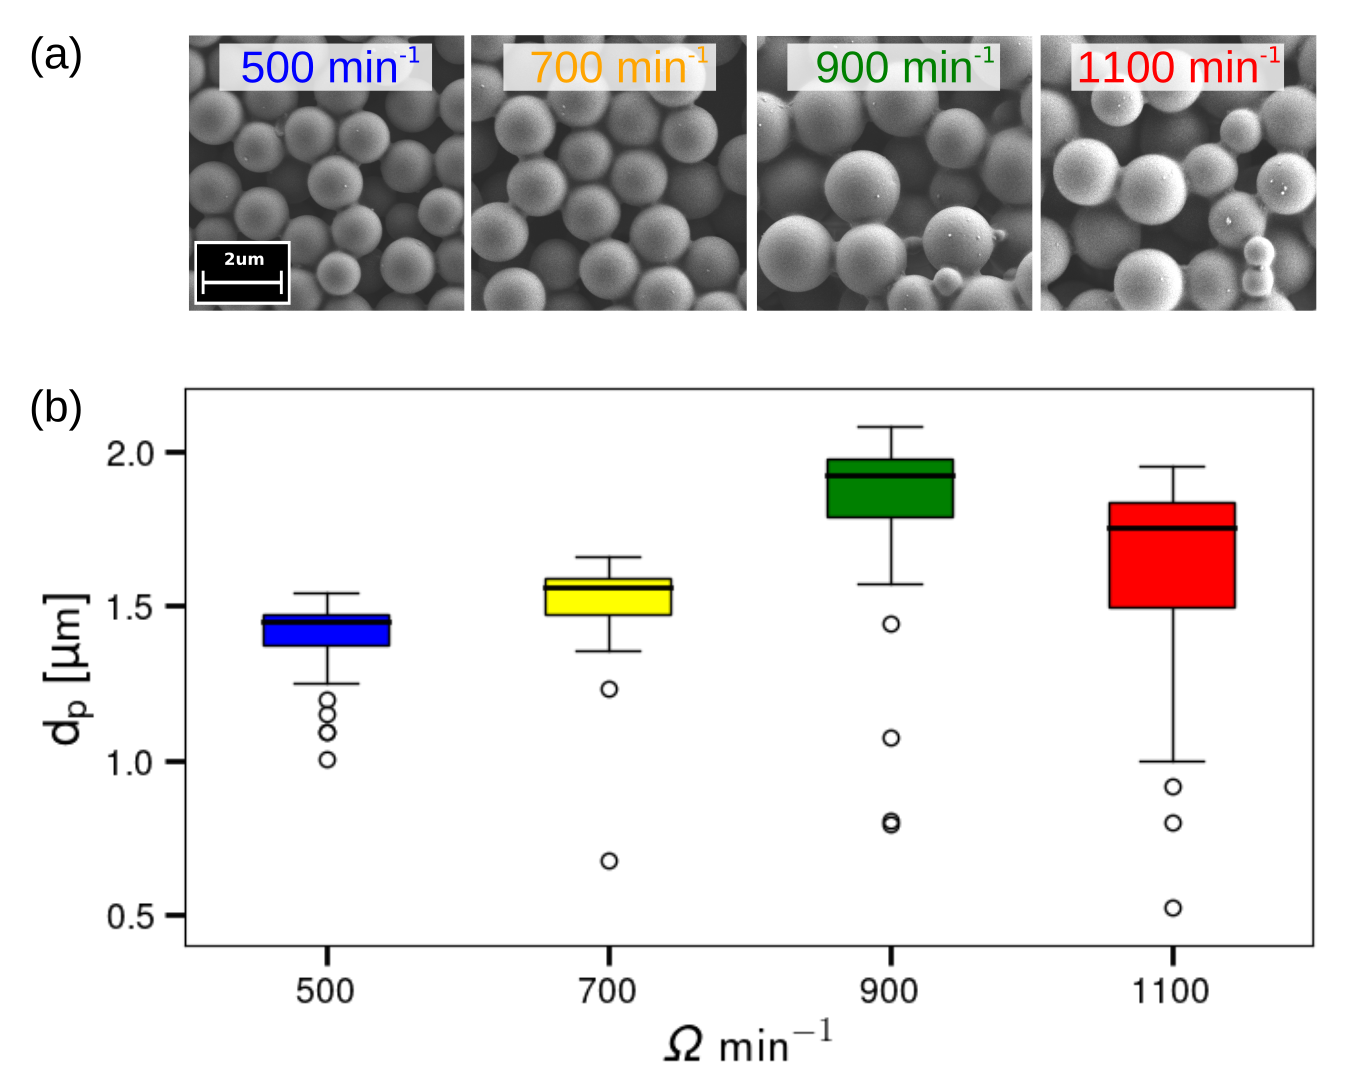
\includegraphics[width=\columnwidth]{sem_stir_analysis}
    \caption{(a) Cropped and scaled SEM images of the polymerized TPM spheres whose
      samples were stirred at \num{500}, \num{700}, \num{900}, and \SI{1100}{\minute^{-1}}.
      (b)  Box and whisker plots summarize the diameters of colloidal spheres estimated from
      SEM digital images. Each rectangular box extends from the first quartile, $Q_1$, to
      the third quartile, $Q_3$, of the data; within each box a black line represents the median;
      the upper whisker extends to largest observed diameter less than $Q_3 + 1.5\, (Q_3 - Q_1)$;
      the lower whisker extends to the smallest observed diameter greater than $Q_1 - 1.5\, (Q_3 - Q_1)$;
      data beyond the whiskers are plotted as open circles. }
    \label{fig:sem_stir_rate}
\end{figure}

Each of the four samples of polymerized spheres were imaged with an SEM;
Fig.~\ref{fig:sem_stir_rate}(a) illustrates cropped and scaled snippets of SEM
images for each sample. Estimates for the diameters for each sample
were produced by drawing tight-fitting ovals around polymer spheres in the image;
the average of the each oval's minor and major axis gave an estimate for the
associated sphere's diameter. This hand-drawing procedure produced estimates
for \num{50} spheres for each sample, providing a total of \num{200} estimates
and are summarized in Fig.~\ref{fig:sem_stir_rate}(b).
The average particle diameters were \SI{1.40}{\um}, \SI{1.52}{\um},
\SI{1.82}{\um}, and \SI{1.64}{\um} for stirring rates \num{500}, \num{700}, \num{900}, and
\SI{1100}{\minute^{-1}} respectively; similarly, the standard deviation of particle diameters
were \SI{0.12}{\um}, \SI{0.13}{\um}, \SI{0.28}{\um}, and \SI{0.32}{\um}.

\begin{figure}
    \centering
    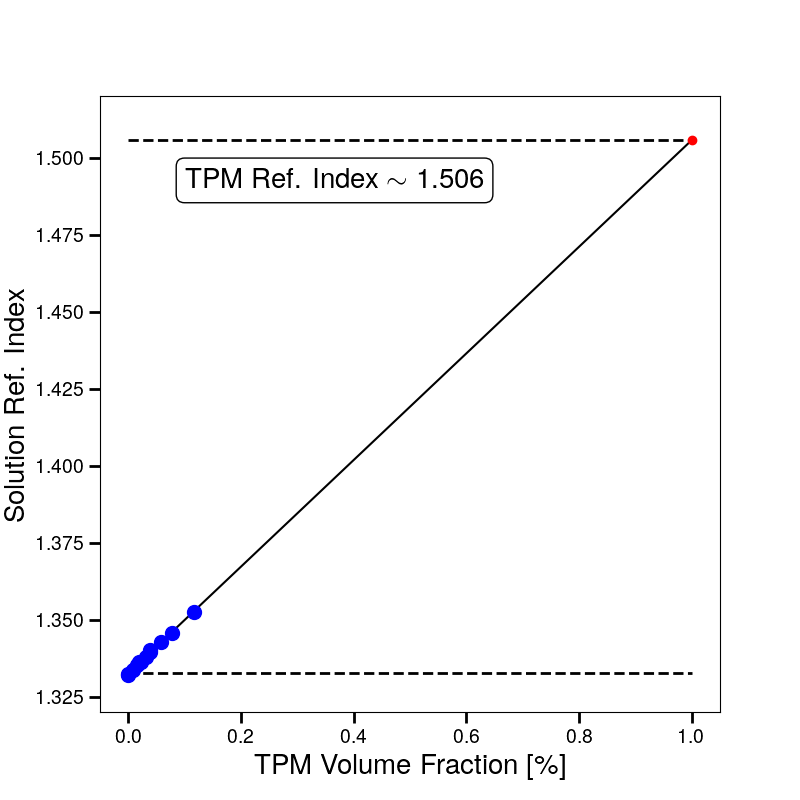
\includegraphics[width=0.7\columnwidth]{abbe_madness}
    \caption{A scatterplot of the measured refractive index of \num{12} solutions with differing
      volume fractions of TPM. A linear fit to the data, represented as a solid black line,
      provides an estimate of the refractive index of polymerized TPM, $n_{\text{p}}$, represented as a red dot.
      The light blue region encompassing the linear fit denotes a $\SI{95}{\percent}$ prediction interval
      that bounds the error in our extrapolated estimate of refractive index.
      The lower dashed line represents the refractive index of water at \SI{532}{\nm}.}
    \label{fig:abbe}
\end{figure}

Two similarly prepared samples of TPM spheres were used to estimate the refractive
index, $n_p$, of the colloidal spheres.
Each sample was diluted to \num{5} different volume fractions to provide a total of
\num{12} different suspensions, including the two stock solutions. The refractive index of each
suspension was measured with an Abbe refractometer;
the results are summarized in Fig.~\ref{fig:abbe}.
By assuming a linear relationship between volume fraction and suspension refractive
index, we estimate the refractive index of TPM colloidal spheres to be \SI{1.506}{}
with a \SI{95}{\percent} confidence that lies in the range $\left ( 1.499, 1.513 \right ).

%In general, there exists a linear relationship between the volume fraction of colloidal
%spheres, $\phi$, and the suspension refractive index. We estimate the refractive
%index of polymerized TPM spheres by extrapolating from our low volume fraction data
%up to a volume fraction of \num{1}. Our estimate is bounded by a $\SI{95}{\percent}$
%prediction interval given by
%\begin{align}
%  \text{Prediction Interval} &= \hat{n_{\text{p}}} \pm t_{\alpha/2, N-2} \, \sqrt{ S^2 +  S_{\hat{n_{\text{p}}}}^2} \\
%  S_{\hat{n_{\text{p}}}}^2 &= S^2 \, \left ( \frac{1}{N} + \frac{\left ( \phi^* - \bar{\phi_i} \right )}{Y} \right )\\ 
%  S^2 &= \frac{\sum_i \left (n_i - (m \, \phi + b )\right )^2}{N-1}\\
%  S_{\phi\phi} &= \sum_i \phi_i^2 - \left ( \sum_i \phi_i \right )^2 /N
%\end{align}

\begin{figure}
    \centering
    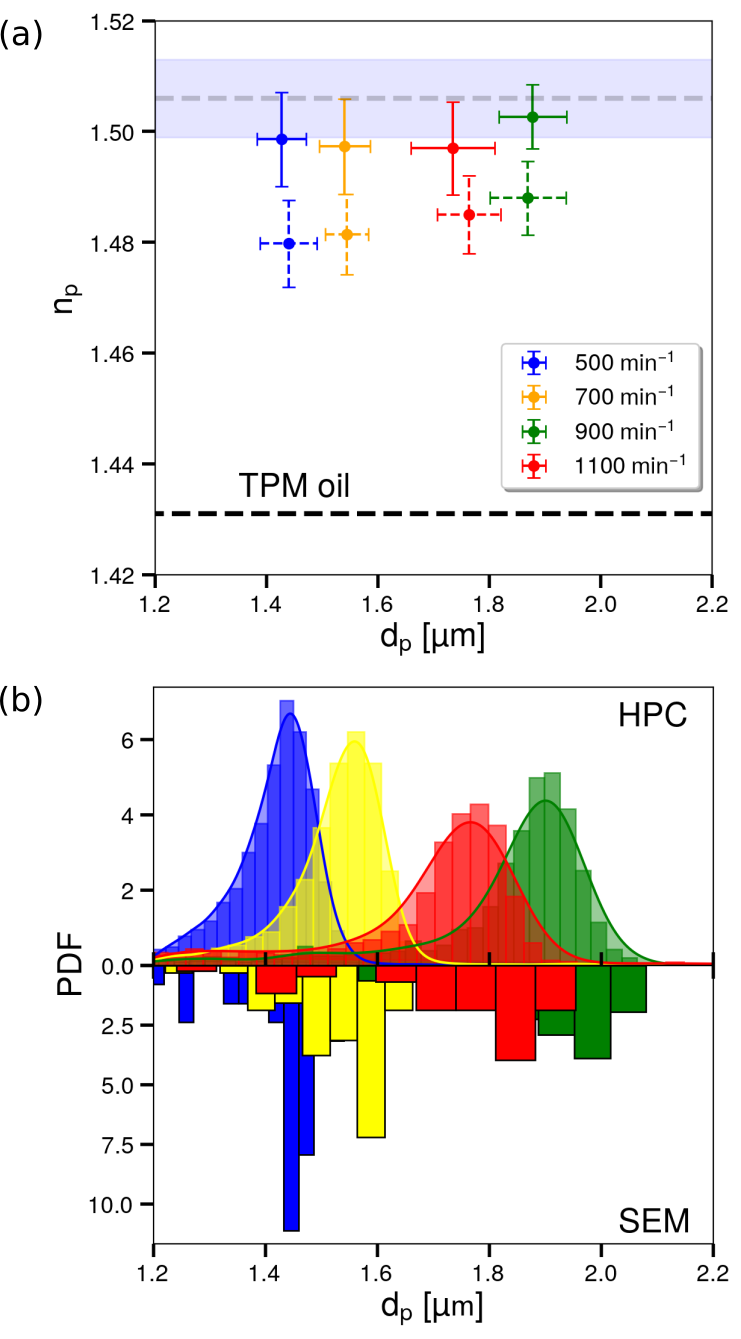
\includegraphics[width=0.6\columnwidth]{orthogonal_vs_hpc}
    \caption{(a) The result of HPC analysis for the unpolymerized and polymerized
      emulsions stirred at \num{4} different rates. Solid-lines represent the polymerized
      spheres; dashed-lines represent the unpolymerized droplets; color differentiates the sample by
      spin rate. Each dot represents the
      average diameter and refractive index for a sample. Error bars are set by a single
      median absolute deviation of the measured property for a given sample. The dashed
      black line provides reference to the refractive index of monomeric TPM oil. (b) Probability
      distributions of diameter as measured by HPC and by SEM analysis. HPC samples the diameter
      densely enough to allow reasonable kernel density estimation.}
    \label{fig:hpc_stir_rate}
\end{figure}


The result of holographic particle characterization for the \num{4} polymerized samples
and the \num{4} unpolymerized samples are summarized in Fig.~\ref{fig:hpc_stir_rate}(b).
Each dot represents the average size and refractive index for the associated sample. Error
bars represent the single median absolute deviation of the associated property.
The unpolymerized droplets, represented with dashed error, bars have a systematically
lower refractive index than the polymerized droplets, represented with solid error bars.
Polymerization changes the chemical makeup of the droplet and generally increases the
density; %% FIXME: Add citation.
both processes might reasonably account for the observed increase.
Both values greatly exceed the refractive index of bulk TPM oil, which is indicated by
a dashed line in Fig.~\ref{fig:synthesis_stir_rate}(b).
Hydrolysis and oligomerization of TPM oil account for three quarters of
the total change.

% comment on how close the HPC result is to the abbe result.
% comment on the slight shrinkage of particles but the closeness of SEM and HPC
% comment on the amount of data and the ease of preparation in comparing these
% techniques to HPC.



\subsection{Effect of heat bath exposure time}

This synthesis of TPM employs heat-activated free-radical initiators to polymerize TPM droplets:
time spent thermally coupled to a heat bath greatly accelerates polymerization.
As observed in Fig.~\ref{fig:synthesis_stir_rate}, the polymerization of
liquid TPM droplets can induce a shift of approximately \SI{0.02}{} in refractive index
which is well within the precision of the xSight.  Because the refractive index
of a material is a function of its composition \cite{wang15},
refractive index serves as a proxy for the degree of
polymerization of a sample.  Holographic particle
characterization is uniquely poised to probe the time dependent polymerization of TPM as
it can monitor the refractive index of individual spheres \emph{in situ}.

We investigate the polymerization rate of TPM droplets by regularly sampling a
suspension undergoing polymerization and characterizing each drawn sample with HPC.
Specifically, the suspension consists of an emulsion of TPM droplets
and the initiator AIBN. The suspension is continuously stirred at \SI{1100}{\min^{-1}}
and is thermally coupled to a heat bath set at \SI{80}{\degreeCelsius}.
We drew \SI{1}{\ul} of the suspennumon after \num{0}, \num{5}, \num{10}, \num{15},
\num{20}, \num{40}, and \SI{60}{\min}. Each sample is added to \SI{1}{\ml} of
room temperature DI water, which effectively arrests any continued polymerization.
Each sample is then immediately characterized by the xSight. Figure ~\ref{fig:heat_size_time}
depicts the result of this chacterization.
%XXX (Add conclusions about polymerization time- only takes maybe 15 min?)


\begin{figure}
    \centering
    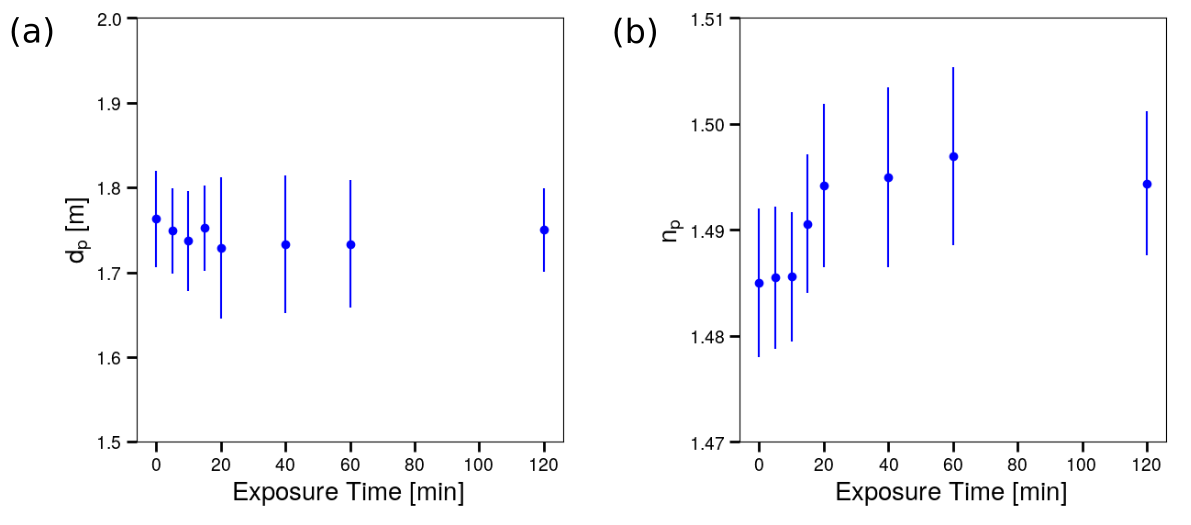
\includegraphics[width=\columnwidth]{synthesis_heat_bath}
    \caption{Particle properties after heat bath exposure times of \num{0}, \num{5},
      \num{10}, \num{15}, \num{20}, \num{40}, and \SI{60}{\min}.
      (a) The average size and (b) refractive index of particles as a function
      of heat bath exposure time. Error bars indicate a single median absolute deviation
      of the associated property.}
    \label{fig:heat_size_time}
\end{figure}

Fig.~\ref{fig:heat_size_time}(a) demonstrates that any changes in size are below
the polydispersity in size. Fig.~\ref{fig:heat_size_time}(b), however, demonstrates
a large shift in refractive index. The first ten minutes are nearly identical;
presumably this is while the suspension is equilibrating with the heat bath.
At \num{15} and \SI{20}{\min} the refractive index significantly increases.
van der Wel \emph{et. al} \cite{vanderwel17} suggest heating the suspension
for \SI{2}{\hour} to ensure the sample has sufficiently polymerized and is
stable. Our analysis suggests that a much shorter time may suffice although
we have not confirmed the resulting stability of the polymerized sample.



\subsection{Effect of stoichiometry and choice of free-radical initiator}

To probe the variables of droplet formation, we make four batches of droplets.
In each case we hold the volume of water, \SI{5}{\milli \liter} constant 
and vary the amounts of TPM and ammonia. Batches A and B each had 
\SI{100}{\micro\liter} of TPM with \si{10} and \SI{20}{\micro\liter} of 
ammonia added, respectively. Batches C and D had \SI{150}{\micro\liter}, 
again with \si{10} and \SI{20}{\micro\liter} of ammonia, respectively. 
\SI{0.1}{\percent} sodium docecyl sulfate (SDS) was introduced to
each sample to suppress aggregation. Through this, we can observe the effects of
varying the amount of TPM and the pH on the size of the resulting droplets.
This gives 
% XXX (Add conclusions about initiator- does not seem to matter)

Next, we observe the effect of using different free radical initiators 
to polymerize the particles. Two water-insoluble initiators, AIBN and
\num{1},\num{1}'-azobis(cyclohexanecarbonitrile) (ACHN), and two water-soluble 
initiators, potassium persulfate (KPS) and ammonium persulfate APS), were 
used.

To compare initiators, one \SI{5}{\milli \liter} suspension of emulsion droplets is
made in a \SI{12}{\milli \liter} vial and then equally divided into five
\SI{1.5}{\milli \liter} microcentrifuge tubes. One tube was left unpolymerized. The
other four tubes were then polymerized at \SI{80}{\celsius} 
for \SI{12}{\hour} on a shaker at \SI{750}{\minute^{-1}} % XXX Again, rpm vs mins^{-1}
to prevent sedimentation.
We added a different free radical initiator to each tube and repeated the process with four
different emulsions for a total of 
\num{16} measurements to ensure that any observations were the result of the 
initiator used and not of the particular protocol used to make the emulsion.


% Van Der Wel et. al suggest that the density increases by 1.07 during polymerization.
% IF the mass stays the same, this corresponds to a 2% decrease in radius.
% For a 1.5 um diameter TPM sphere, a 2% decrease reduces the size to 1.46 um.
% That would be visible in our 

\begin{figure}
    \centering
    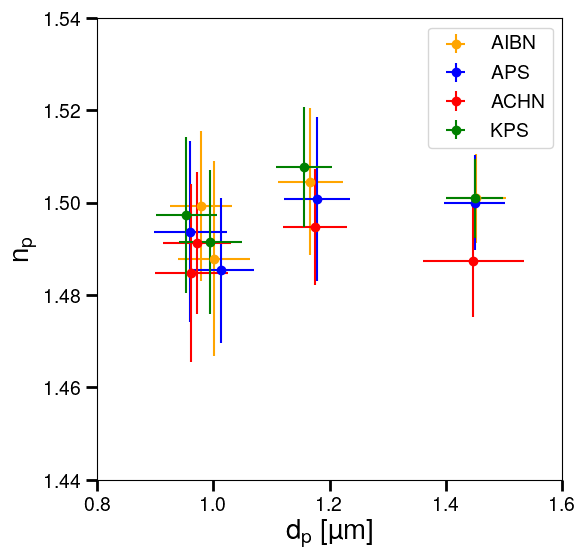
\includegraphics[width=0.75\columnwidth]{may_data_summary.png}
    \caption{The refractive index and diameter of 16 samples of 
    polymerized TPM.}
    \label{fig:initiator_data}
\end{figure}

In making the \si{16} sets of particles to look at the effect of initiator on 
the particles, we can also make observations about the effects of varying 
the amount of TPM and the pH on the size of the resulting droplets. To hold 
the pH constant, we can compare sample A to C and sample B to D. This gives 
the fairly intuitive result that increasing the amount of TPM increases the 
size of the final droplet. Holding the amount of TPM constant and varying 
the pH, which means comparing A to B and C to D, shows that increasing the 
pH of the environment during droplet formation decreases the size of the 
final droplet. This is less intuitive but perhaps not surprising, as the pH 
affects the rate at which oligomers form and therefore the rate of droplet 
formation. This leads to more nucleation sites and therefore smaller droplets 
for the same volume of material. 

Comparing batches A to C, each with \SI{100}{\micro \liter} of TPM monomer, and B to D with
\SI{150}{\micro \liter}, gives the somewhat intuitive result that increasing the amount of TPM
monomer increases the size of the final droplet. On the other hand, comparing A to B with
\SI{10}{\micro \liter} ammonia and C to D with \SI{15}{\micro \liter} ammonia shows that
increasing the pH of the environment during droplet formation decreases the size of the 
final droplet. This is less intuitive but perhaps not surprising, as the pH 
affects the rate at which oligomers form and, therefore, the rate of droplet 
formation. Increasing the pH results in more nucleation sites and therefore smaller droplets 
for the same volume of material. 

Under certain conditions, TPM droplets are known to form dimpled spheres when polymerized with
the water-soluble initiators APS and KPS due to the ejection of low molecular weight oligomers
(citation- I forget which of Stefano's papers?). Therefore, one might think that TPM spheres
polymerized with these initiators would be made of on average higher molecular weight oligomers
and have a higher refractive index than pa. However, under the conditions observed here where no
dimple was formed, there was no observable difference in particle size or refractive index between
the initiators used.

\section{Discussion}

\section{Acknowledgment}

This work was supported primarily by the MRSEC program of
the National Science Foundation through Award Number DMR-1420073.
Additional support was provided by the SBIR program of the
National Science Foundation through Award Number IPP-1519057.
The FESEM was purchased with financial support from the MRI program
of the National Science Foundation under Award DMR-0923251.

\% FIXME David please check the acknowledgment
